\begin{frame}
    \frametitle{Научная новизна}
    \footnotesize
    \begin{itemize}
        \item Впервые предложена и исследована стохастическая модель системы радиочастотной идентификации ТС, учитывающая скорость движения RFID-меток, расположенных на номерных знаках автомобилей, а также различные сценарии проведения опроса и сбора данных с меток.
        \item Разработан комплекс новых аналитических и имитационных моделей для анализа вероятности идентификации ТС, учитывающих особенности логического и физического уровней протокола стандарта EPC Class 1 Gen.2, и особенности распространения радиосигналов между RFID-меткой и считывателем.
        \item Предложена новая методика моделирования многошаговых беспроводных сетей с помощью тандемных сетей массового обслуживания, учитывающая особенности трафика и интерференции в каналах связи.
        \item Разработан оригинальный метод вычисления оценок характеристик многофазных систем массового обслуживания большой размерности с коррелированными входными потоками и распределениями обслуживания фазового типа.
        \item Разработана архитектура и реализована новая распределенная система управления RFID-считывателями, предназначенная для организации сбора данных об идентифицированных транспортных средствах.
        \item Проведена обработка экспериментальных данных, полученных при опытных внедрениях разработанной системы в г. Казань и на ЦКАД в Московской области, показавшая высокое совпадение с теоретическими результатами диссертации.
    \end{itemize}
\end{frame}
\note{
    Проговаривается вслух научная новизна
}

\begin{frame}[allowframebreaks]
    \frametitle{Практическая значимость}
    \small
    \begin{itemize}
        \item Аналитические и имитационные модели и методы, предложенные в диссертации, могут эффективно использоваться для оценки производительности систем радиочастотной идентификации автомобилей и широкополосных беспроводных сетей.
        \item Распределенная система управления считывателями и программное обеспечение, описанные в работе, использовались в трех экспериментальных внедрениях на автодорогах в г. Казань и Московской области.
        \item Практическая значимость диссертационной работы подтверждается актами о внедрении, полученными от Государственного бюджетного учреждения <<Безопасность дорожного движения>> (г. Казань) и ПАО <<Микрон>>.
    \end{itemize}
    \framebreak
    Результаты работы также были использованы в исследованиях, проводимых по следующим грантам:
    \footnotesize
    \begin{itemize}
        \item Контракт c Министерством образования и науки РФ № 14.514.11.4071 в рамках федеральной целевой программы <<Исследования и разработки по приоритетным направлениям развития научно-технологического комплекса России на 2007-2013 годы>>.
        \item Соглашение с Министерством образования и науки РФ о предоставлении субсидии от 22.10.2014 г. № 14.613.21.0020 в рамках федеральной целевой программы <<Исследования и разработки по приоритетным направлениям развития научно-технологического комплекса на 2014-2020 годы>>.
        \item Грант Российского научного фонда (РНФ) № 16-49-02021.
        \item Грант РФФИ № 13-07-00737.
        \item Гранты РФФИ (международный проект РФФИ "--- БРФФИ) № 14-07-90015, 16-57-00130
    \end{itemize}
\end{frame}
\note{
    Проговариваются вслух научная и практическая значимость
}

\begin{frame}
    \frametitle{Акты о внедрении}
    \begin{minipage}[t]{0.49\linewidth}
        \includegraphics[width=\linewidth]{act_bdd.pdf}
    \end{minipage}
    \hfill
    \begin{minipage}[t]{0.49\linewidth}
        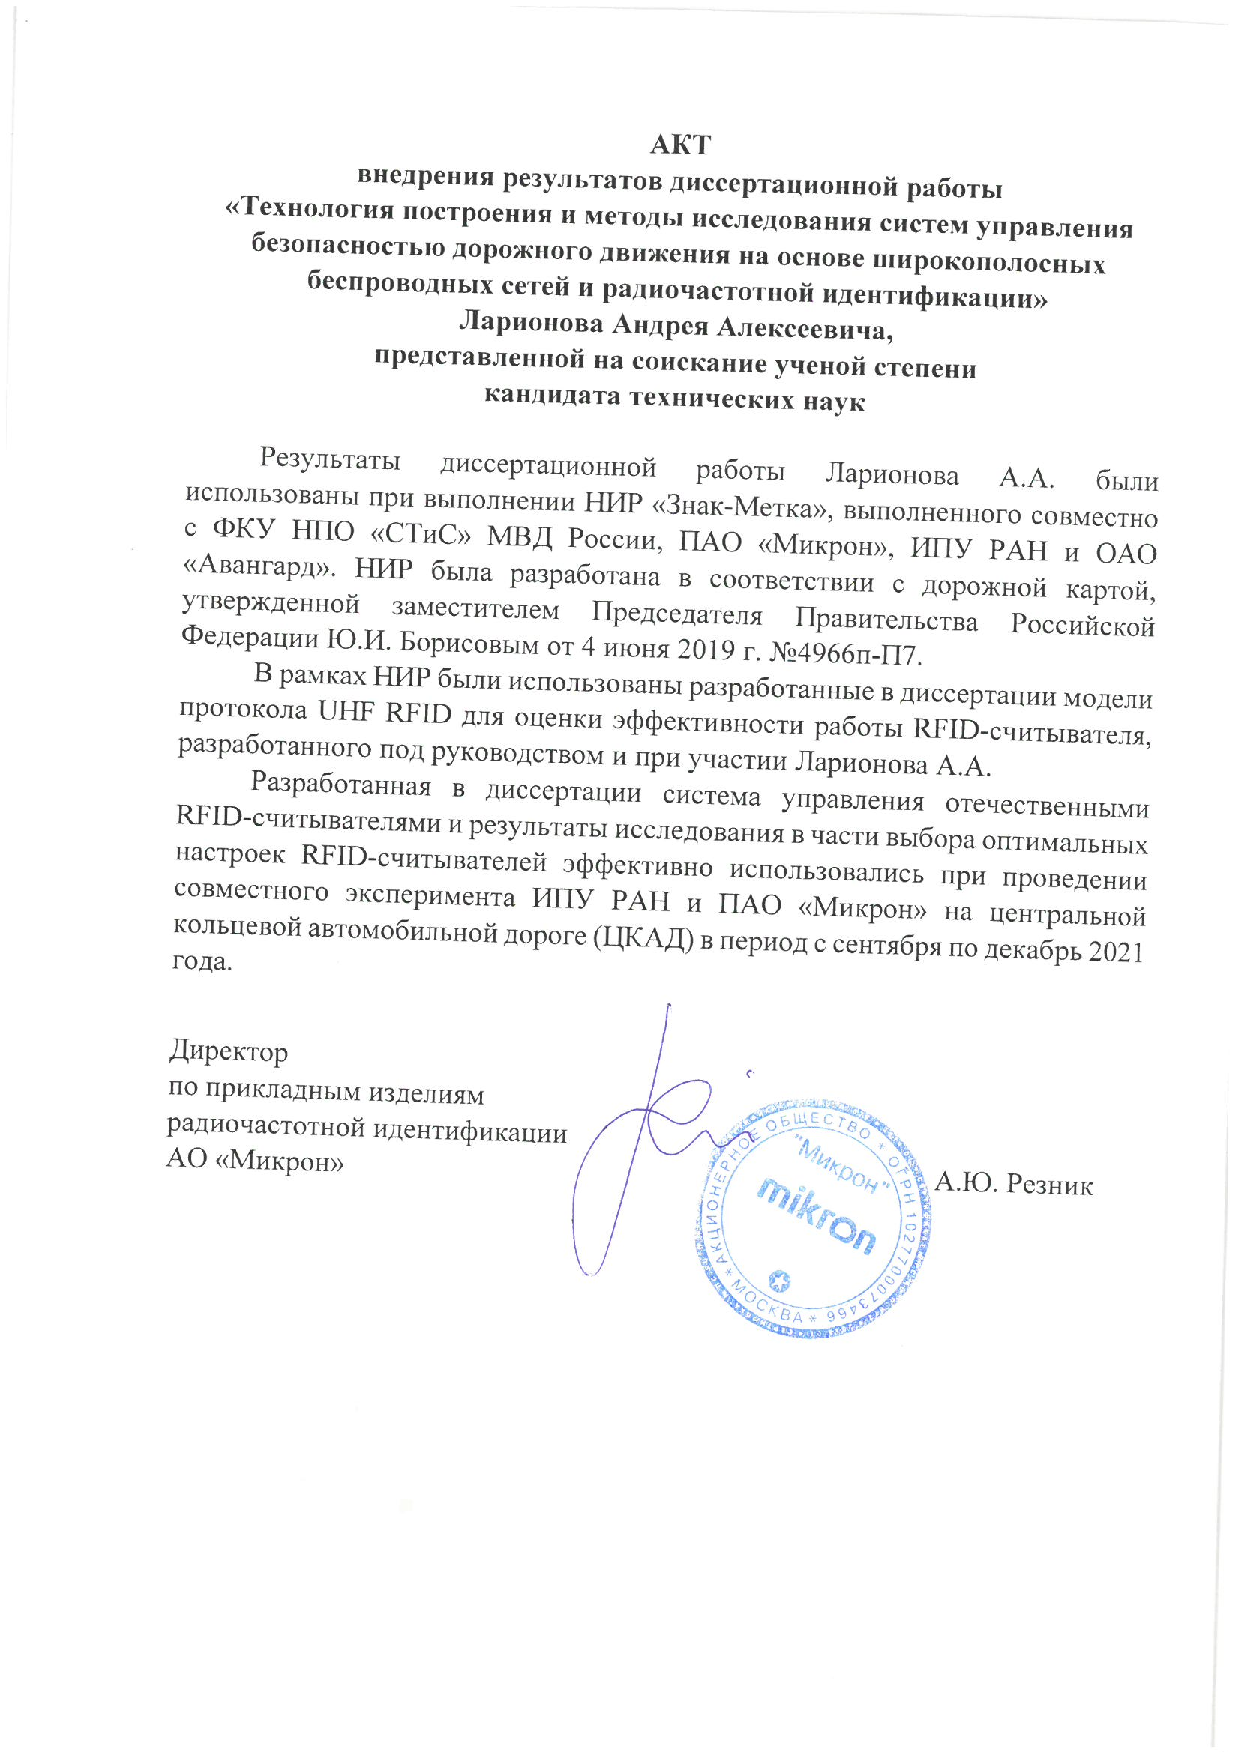
\includegraphics[width=\linewidth]{act_mikron.pdf}
    \end{minipage}
\end{frame}
\note{
    Были получены акты о внедрении от ГБУ <<Безопасность дорожного движения>> (город Казань) и от ПАО <<Микрон>>.
}

\begin{frame}[t,allowframebreaks,plain,noframenumbering] % публикации на нескольких страницах
    \frametitle{Основные публикации}
    \setbeamertemplate{enumerate items}[default]
    \footnotesize
    \begin{enumerate}
        \item \textbf{A. Larionov}, R. Ivanov, V. Vishnevsky. UHF RFID in Automatic Vehicle Identification: Analysis and Simulation // IEEE Journal of Radio Frequency Identification. "--- IEEE, 2017. "--- 3. "--- Vol. 1, no. 1. "--- Pp. 3--12.
        \item Performance Evaluation of the Priority Multi-Server System MMAP/PH/M/N Using Machine Learning Methods / V. Vishnevsky, V. Klimenok, A. Sokolov, \textbf{A. Larionov} // Mathematics. "--- MDPI, 2021. "--- Vol. 9, no. 24.
        \item Review of methodology and design of broadband wireless networks with linear topology / V. Vishnevsky, A. Krishnamoorthy, D. Kozyrev, \textbf{A. Larionov} // Indian Journal of Pure and Applied Mathematics. "--- Springer, 2016. "--- Vol. 47, no. 2 "--- Pp. 329--342.
        \item Методы исследования и проектирования широкополосных беспроводных сетей вдоль протяженных транспортных магистралей / В.М. Вишневский, А. Кришнамурти, Д.В. Козырев, \textbf{А.А. Ларионов}, Р.Е. Иванов // T-Comm: Телекоммуникации и транспорт. "--- Москва: Медиа ПАБЛИШЕР, 2015. "--- Т.9, №~5. "--- С.~9--15.
        \item В.М. Вишневский, \textbf{А.А. Ларионов}, О.В. Семёнова. Оценка производительности высокоскоростной беспроводной тандемной сети с использованием каналов сантиметрового и миллиметрового диапазона радиоволн в системах управления безопасностью дорожного движения // Проблемы управления. "--- Москва: Сенсидат-Плюс, 2013. "--- Т.~4. "--- С.~50--56.
        \item Новое поколение систем безопасности на автодорогах и их применение в интеллектуальных транспортных системах / В.М. Вишневский, Р.Н. Минниханов, А.Н. Дудин, В.И. Клименок, \textbf{А.А. Ларионов} // Информационные технологии и вычислительные системы. "--- Москва: Издательство ИСА РАН, 2013. "--- Т.~4. "--- С.~80--89.
        \item В.М. Вишневский, \textbf{А.А. Ларионов}, Ю.В. Целикин. Анализ и исследование методов проектирования автоматизированных систем безопасности на автодорогах с использованием новых широкополосных беспроводных средств и RFID-технологий // T-Comm: Телекоммуникации и транспорт. "--- Москва: Медиа ПАБЛИШЕР, 2012. "--- T.~7. "--- С.~48--54.
        \item V. Vishnevsky, \textbf{A. Larionov}. Stochastic Multiphase Models and Their Application for Analysis of End-to-End Delays in Wireless Multihop Networks // Applied Probability and Stochastic Processes. Infosys Science Foundation Series. "--- Springer, 2020. "--- Pp. 457--471.
        \item A Multiphase Queueing Model for Performance Analysis of a Multi-hop IEEE 802.11 Wireless Network with DCF Channel Access / \textbf{A. Larionov}, V. Vishnevsky, O. Semenova, A. Dudin // Information Technologies and Mathematical Modelling. Queueing Theory and Applications. ITMM 2019. Communications in Computer and Information Science. "--- Springer, 2019. "--- Vol.~1109. "--- Pp.~162--176.
        \item \textbf{A. Larionov}, R. Ivanov, V. Vishnevsky. A stochastic model for the analysis of session and power switching effects on the performance of UHF RFID system with mobile tags // 2018 IEEE International Conference on RFID (RFID). "--- Orlando: IEEE, 2018. "--- Pp.~1--8.
        \item I.R. Lavrukhin, \textbf{A.A. Larionov}, A.A. Yelizarov. Analysis and Modeling of the Protocol of Radio Frequency Identification of Vehicles on Road Stations // 2018 System of Signal Synchronization, Generating and Processing in Telecommunications (SYNCHROINFO). "--- IEEE, 2018. "--- 7. "--- Pp.~1--5.
        \item V. Vishnevsky, \textbf{A. Larionov}, R. Ivanov. Applying UHF RFID for Vehicle Identification: Protocol and Propagation Simulation // 2017 IEEE International Conference on RFID (RFID). "--- Phoenix, AZ: IEEE, 2017. "--- 5. "--- Pp.~73-80.
        \item Estimation of IEEE 802.11 DCF access performance in wireless networks with linear topology using PH service time approximations and MAP input / \textbf{A.A. Larionov}, V.M. Vishnevsky, R.E. Ivanov, O.V. Semenova // Proceedings of the 11th IEEE International Conference on Application of Information and Communication Technologies (AICT'2017, Moscow). "--- Vol.2 "--- Moscow: IEEE, 2017. "--- Pp.~85--89.
        \item State Reduction in Analysis of a Tandem Queueing System with Correlated Arrivals / V.M. Vishnevsky, \textbf{A.A. Larionov}, O.V. Semenova, R.E. Ivanov // Communications in Computer and Information Science. "--- Vol.~800. "--- Springer, 2017. "--- Pp.~215--230.
        \item V.M. Vishnevsky, \textbf{A.A. Larionov}, R.E. Ivanov. An open queueing network with a correlated input arrival process for broadband wireless network performance evaluation // Communications in Computer and Information Science. "--- Vol.~638. "--- Springer, 2016. "--- Pp.~354--365.
        \item Methods of performance evaluation of broadband wireless networks along the long transport routes / V. Vishnevsky, A. Dudin, D. Kozyrev, \textbf{A. Larionov} // Communications in Computer and Information Science. "--- Vol.~601. "--- Springer, 2016. "--- Pp.~72--85.
        \item V. Vishnevsky, \textbf{A. Larionov}, R. Ivanov. Analysis and Simulation of UHF RFID Vehicle Identification System // Communications in Computer and Information Science. "--- Vol.~678. "--- Springer, 2016 "--- Pp.~35--46.
        \item V. Vishnevsky, \textbf{A. Larionov}, R. Ivanov. Architecture of application platform for RFID-enabled traffic law enforcement system // 2014 7th International Workshop on Communication Technologies for Vehicles, Nets4Cars-Fall 2014. "--- IEEE, 2014. "--- Pp.~45-49.
        \item V. Vishnevsky, \textbf{A. Larionov}. Design concepts of an application platform for traffic law enforcement and vehicles registration comprising RFID technology // 2012 IEEE International Conference on RFID-Technologies and Applications, RFID-TA 2012. "--- IEEE, 2012. "--- Pp.~148--153.
    \end{enumerate}
\end{frame}

% % \begin{frame} % публикации на одной странице
% \begin{frame}[t,allowframebreaks,plain,noframenumbering] % публикации на нескольких страницах
%     \frametitle{Основные публикации}

%     \nocite{RFID_JRFID2017}
%     \nocite{WINET_IJPAM2016}
%     \nocite{WINET_TCOMM2015}
%     \nocite{QS_JPU2013}
%     \nocite{QS_JITCS2013}
%     \nocite{QS_TCOMM2012}

%     %
%     %% authorwos
%     % \nocite{wosbib1}%

%     \nocite{QS_ICAAPSP2020}
%     \nocite{QS_ITMM2019}
%     \nocite{RFID_IEEERFID2018}
%     \nocite{RFID_SYNCHROINFO2018}
%     \nocite{RFID_IEEERFID2017}
%     \nocite{QS_AICT2017}
%     \nocite{QS_ITMM2017}
%     \nocite{QS_ITMM2016}
%     \nocite{QS_DCCN2016_CCIS}
%     \nocite{RFID_DCCN2016_CCIS}
%     \nocite{RFIDCTRL_NETS2CARS2014}
%     \nocite{RFIDTA2012}

%     % \nocite{Fedotov2020}
%     % \nocite{Fedotov2020a}
%     % \nocite{RFID_VSPU2019}
%     % \nocite{WINET_DCCN2018}
%     % \nocite{RFIDCTRL_DCCN2017}
%     % \nocite{RFID_DCCN2015_RUS}
%     % \nocite{QS_DCCN2015}
%     % \nocite{QS_ITTMM2015}
%     % \nocite{RFIDCTRL_VSPU2014}
%     % \nocite{RFID_DCCN2013_RUS}

%     %
%     %% authorscopus
%     % \nocite{scbib1}%
%     %
%     %% authorconf
%     % \nocite{confbib1}%
%     % \nocite{confbib2}%
%     %
%     %% authorother
%     % \nocite{bib1}%
%     % \nocite{bib2}%
%     \ifnumequal{\value{bibliosel}}{0}{
%         \insertbiblioauthor
%     }{
%         \printbibliography%
%     }
% \end{frame}
% \note{
%     Результаты работы опубликованы в N печатных изданиях,
%     в~т.\:ч. M реферируемых изданиях.
% }

\begin{frame}[plain,noframenumbering]
    \frametitle{Участие в конференциях}
    \footnotesize
    \begin{itemize}
        \item IEEE RFID, 2017, 2018 (США);
        \item Международный форум Kazan Digital Week 2020 (Казань);
        \item International conference on Advances in Applied Probability and Stochastic Processes 2019 (ICAAP \& SP 2019; Индия, Коттаям);
        \item Всероссийские совещания по проблемам управления (ВСПУ 2019, ВСПУ 2014; Москва, ИПУ РАН);
        \item Международная конференция им. А.Ф. Терпугова Информационные технологии и математическое моделирование (ИТММ 2016, 2017, 2019, 2021; Россия);
        \item 11th IEEE International Conference on Application of Information and Communication Technologies (IEEE AICT 2017; Москва, ИПУ РАН);
        \item Международная конференция Распределенные компьютерные и телекоммуникационные сети: управление, вычисление, связь (DCCN 2013, 2015, 2016, 2017, 2018; Москва);
        \item 7th International Workshop on Communication Technologies for Vehicles (Nets4Cars-Fall 2014; Санкт-Петербург);
        \item 2012 International Conference on RFID-Technology and Applications (IEEE RFID-TA 2012; Франция);
        \item Всероссийская конференция Информационно-телекоммуникационные технологии и математическое моделирование высокотехнологичных систем (ИТТММ 2015, 2020; Москва, РУДН).
    \end{itemize}
\end{frame}
\note{
    Работа была представлена на 20 конференциях.
}

\begin{frame}[plain, noframenumbering] % последний слайд без оформления
    \begin{center}
        \Huge
        Спасибо за внимание!
    \end{center}
\end{frame}
